
\documentclass[14pt, aspectratio=169]{beamer}
\setbeamertemplate{navigation symbols}{}
\mode<presentation>
{
  \usetheme{Boadilla}
  \usecolortheme{dolphin}
  % or ...

  \setbeamercovered{transparent}
  % or whatever (possibly just delete it)
}

\usepackage[english]{babel}
% or whatever
\usepackage[utf8]{inputenc}
% or whatever
\usepackage{times}
\usepackage[T1]{fontenc}
\usepackage{verbatim}
\usepackage{tikz}
\usetikzlibrary{spy,calc,shapes.misc}
\usepackage{hyperref}




% Or whatever. Note that the encoding and the font should match. If T1
% does not look nice, try deleting the line with the fontenc.

\title[Heteregenous Spillovers in Unconditional Cash Transfer] % (optional, use only with long paper titles)
{Heterogenous Spillovers in Unconditional Cash Transfer}

\author[Abraham, Bechhofer, and Kim] % (optional, use only with lots of authors)
{Abraham, Bechhofer, and Kim }
% - Use the \inst{?} command only if the authors have different
%   affiliation.


%\date[2018.10.16] % (optional)
%{2018.10.16}

\subject{Talks}
% This is only inserted into the PDF information catalog. Can be left
% out.


% If you have a file called "university-logo-filename.xxx", where xxx
% is a graphic format that can be processed by latex or pdflatex,
% resp., then you can add a logo as follows:

% \pgfdeclareimage[height=0.5cm]{university-logo}{university-logo-filename}
% \logo{\pgfuseimage{university-logo}}

% Delete this, if you do not want the table of contents to pop up at
% the beginning of each subsection:
%\AtBeginSubsection[]
%{
%  \begin{frame}<beamer>{Outline}
%    \tableofcontents[currentsection,hideallsubsections]
%  \end{frame}
%}

%\AtBeginSection[]{
%	\begin{frame}
%		\vfill
%		\centering
%		\begin{beamercolorbox}[sep=8pt,center,shadow=true,rounded=true]{title}
%			\usebeamerfont{title}\insertsectionhead\par%
%		\end{beamercolorbox}
%		\vfill
%	\end{frame}
% }

% If you wish to uncover everything in a step-wise fashion, uncomment
% the following command:

%\beamerdefaultoverlayspecification{<+->}
\usepackage{amsmath}
\usepackage{bm}
\usepackage{accents}
\usepackage{float}
\usepackage{stackengine}
\usepackage{rotating}
\usepackage{adjustbox}
\usepackage{graphicx}
\usepackage{kotex}

\setbeamertemplate{itemize items}[default]
\setbeamertemplate{enumerate items}[default]

\let\OLDitemize\itemize
\renewcommand\itemize{\OLDitemize\addtolength{\itemsep}{10pt}}

\let\OLDenumerate\enumerate
\renewcommand\enumerate{\OLDenumerate\addtolength{\itemsep}{10pt}}



\begin{document}

\begin{frame}
  \titlepage
\end{frame}

\begin{frame}{Motivation}
\begin{itemize}
	\item Househofer and Sharpiro (2016): A cluster randomized controlled trial in rural Kenya to study the effect of unconditional cash trasnfers (UCT)
    \item Reported improvements in asset ownership, consumption, income, subjective well-being, and female empowerment for recipients compared to non-recipients in the same village
    \item Study depends on comparability of treated households in the same village (it does on average).
	\item Our question: \\ Does everyone experiences the same amount of spillover?
\end{itemize}
\end{frame}

\begin{frame}{Intervention}
    \begin{itemize}
    	\item Households eligible for study based on a thatched roof criteria
        \item GiveDirectly transfered cash amounting to \$404 PPP
        \item Households are subsistence farmers making \$85 PPP per month
        \item Data from pre-treatment and post-treatment surveys
    \end{itemize}
\end{frame}

\begin{frame}{Intervention}
\begin{figure}[H]
	\centering
	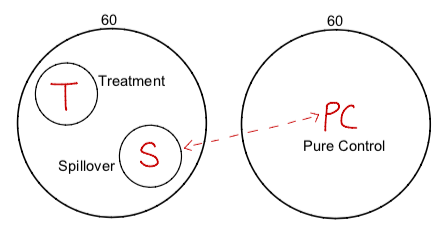
\includegraphics[width=0.9\textwidth]{design.png}
	\caption{Treatment, Spillover, and Pure Control Groups}
\end{figure}
\end{frame}

\begin{frame}{Identifying heterogeneity}
\begin{itemize}
	\item Heterogeneity in linear spillover effects:
	\begin{equation*} \label{eq:interaction}
	Y_{i,v} = \beta_0 + \beta_1 S_v + \beta_2 D_{i,v} + \beta_3 S_v \times  D_{i,v} + \varepsilon_{i,v}
	\end{equation*}

	\item $Y_{i,v}$: Outcome variable of interest
    \item $S_v$: Indicator for living in a treatment village
    \item $D_{i,v}$: Measure of demographic distance of individual $i$

\end{itemize}
\end{frame}

\begin{frame}{Measuring Demographic Distance}
\begin{itemize}
	\item Absolute distance
	$$D_{i,v}  = \frac{|Y_{i,v,t=0} - \bar Y_{v,t=0}|}{\text{SD}_v} $$
	\item Squared deviations from village averages
	$$ D^2_{i,v}= \frac{(Y_{i,v,t=0} - \bar Y_{v,t=0})^2}{\text{SD}_v} $$
	\item Mahalanobis measure
	$$D^\text{M.}_{i,v} = \sqrt{( X_i - {\bar X})' {\hat S}^{-1}_v ( X_i - {\bar X})}  $$
\end{itemize}
\end{frame}

\begin{frame}{Results}
\begin{columns}[T] % align columns
\begin{column}{.35\textwidth}
  \makebox[\linewidth][r]{
    \resizebox{\linewidth}{!}{
    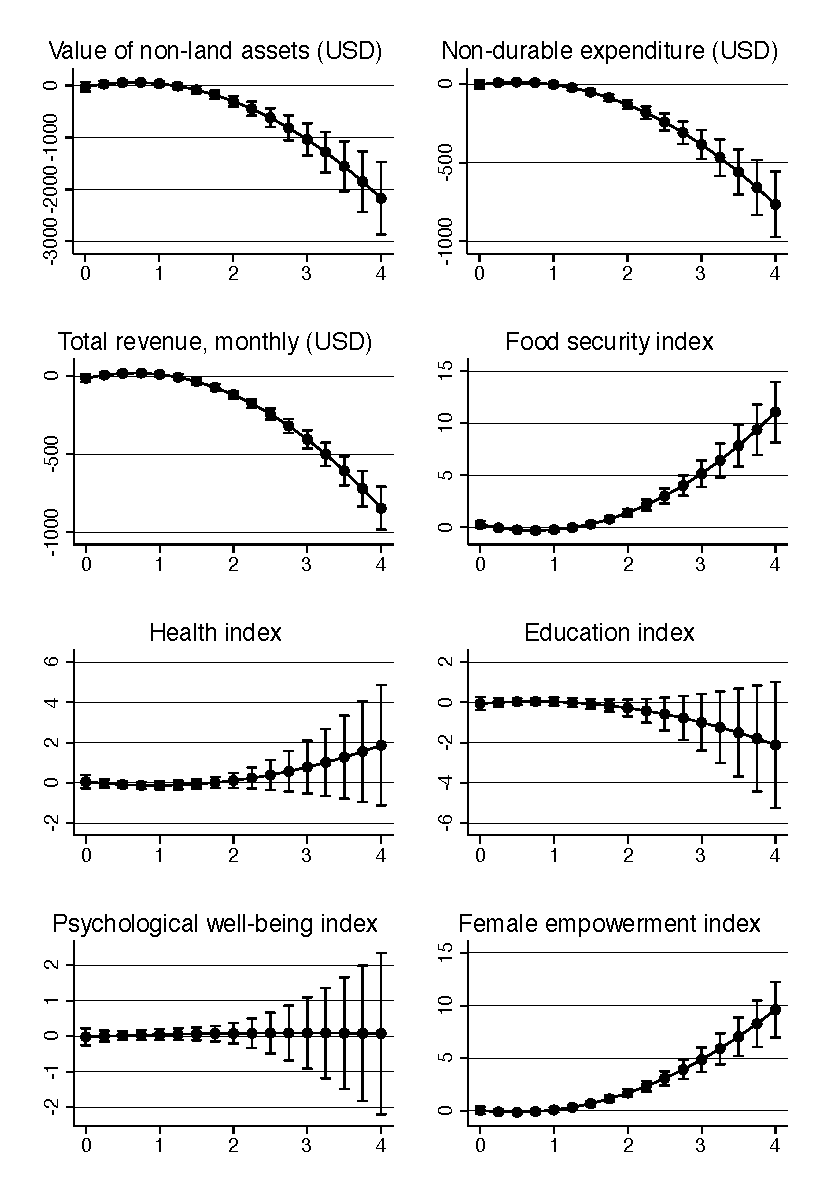
\includegraphics[height=\textheight]{../Figs/indices_ppp_margins.pdf}
    }
  }
  \end{column}%
\hspace{-2.5ex}
\begin{column}{.6\textwidth}
  \makebox[\linewidth][l]{
    \resizebox{\linewidth}{!}{
   \begin{tikzpicture}[spy using outlines={chamfered rectangle,blue,magnification=2,width=18cm, height=8cm, connect spies}]
\node {\includegraphics[page=5, trim={4cm 20cm 0 0}]{../Draft/VSP-draft.pdf}};
\spy on (-4.5,-2.6) in node [right] at (1,9.5);
\end{tikzpicture}

    }
  }
\end{column}%
\end{columns}

\end{frame}

\begin{frame}{Conclusion}

\end{frame}



\end{document}
